\documentclass[a4]{article}
\usepackage[left=2cm,right=3cm,top=1cm,bottom=2cm]{geometry}
\usepackage{graphicx} \usepackage[export]{adjustbox} \usepackage{float}
\usepackage{url} \newcommand{\href}[2]{#2\footnote{\url{#1}}}
\usepackage{amsmath,amssymb,amsfonts}
\newcommand{\eqline}[1]{~\vspace{0.1cm}\\\centerline{$#1$}\vspace{0.1cm}\\}
\newcommand{\defq}{\stackrel {\rm def}{=}}
\newcommand{\tab}{\hphantom{4mm}}

\begin{document} {\huge \bf Programmatoid and neuronoid computations}
\\\centerline{Reference document, v1}
\tableofcontents \newpage

\section{The braincraft challenge}

Let us consider the following digital experimental setup, as described in \href{https://github.com/rougier/braincraft/blob/master/README.md#introduction}{braincraft challenge presentation}.

\subsection{Simplified problem statement}

\centerline{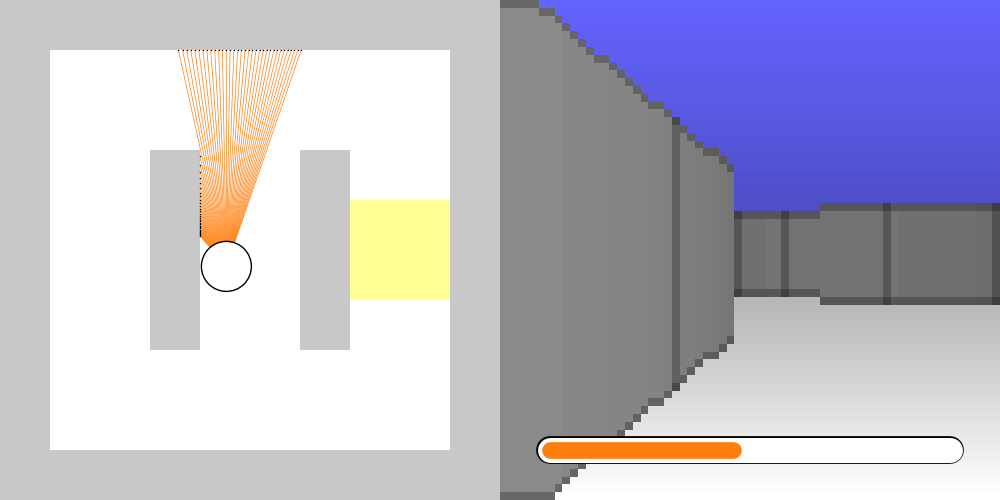
\includegraphics[width=0.9\textwidth]{../../data/debug.png}}

As shown in this figure\footnote{Shared here by courtesy of Nicolas P. Rougier.}, \href{https://github.com/rougier/braincraft}{the braincraft challenge} bot moves at a constant with sensor inputs and one orientation output, it uses some energy and refill this energy on a given yellow location. The 2D space size is $[0, 1] \times [0, 1]$. The bot starts in the middle and oriented at $90°$, i.e., upward.
\eqline{\begin{array}{|ll|l|}
  \hline\multicolumn{3}{|c|}{\mbox{{\bf Input variables}}}\\\hline
  p_l \in [0_{\mbox{wall-hit}}, 1_{\mbox{no-wall}}[ && \mbox{\parbox{5cm}{~\\Leftward proximity, {\small max value of the [0, +30°] range 32 left sensors.\\}}} \\\hline 
  p_r \in [0_{\mbox{wall-hit}}, 1_{\mbox{no-wall}}[ && \mbox{\parbox{5cm}{~\\Rightward proximity, {\small max value of the [-30°, 0] range 32 right sensors.\\}}} \\\hline 
  c_{l\bullet} \in \{0, 1\}, \bullet \in \{b_{\mbox{blue}}, r_{\mbox{red}}\} && \mbox{\parbox{5cm}{~\\Leftward binary red and blue color detectors.\\}}\\\hline 
  c_{r\bullet}  \in \{0, 1\}, \bullet \in \{b_{\mbox{blue}}, r_{\mbox{red}}\} && \mbox{\parbox{5cm}{~\\Rightward binary red and blue color detectors.\\}} \\\hline 
  g_e \in [0_{\mbox{death}}, 1_{\mbox{full}}] && \mbox{\parbox{5cm}{~\\Energy gauge value.\\}} \\\hline 
  \hline \multicolumn{3}{|c|}{\mbox{{\bf Output variables}}}\\\hline
  d_l \in [0, 1_{+ 5^o}] && \mbox{\parbox{5cm}{~\\Left orientation difference.\\}}\\\hline 
  d_r \in [0, 1_{- 5^o}] && \mbox{\parbox{5cm}{~\\Right orientation difference.\\}}\\\hline 
 \end{array}}

With respect to the original braincraft challenge:
\\ \tab - we consider two leftward and rightward ``average'' sensors only,
\\ \tab - color is input as binary variables, and always available,
\\ \tab - the output stands on positive normalized signal,
\\ \tab - the wall hit indicator is not used,


\subsection{Preprocessing}

\subsubsection{Proximity sensors}\begin{description}
\item[Motivation] Simplifies the left-right navigation by compacting the leftward and rightward sensors as a simple pair of input.
\item[Implementation] A simple sum or average could be used, thus using directly a linear combination of the input in afferent units. \\
  \eqline{p_\dagger \leftarrow 1 / 32 \, \sum_{k \in } p[k], \dagger \in \{l_{\mbox{left}}, r_{\mbox{right}},\}}
  where $K_\dagger$ stands for the left or right sensor related $32$ indexes.
We also can use a softmax mechanism as derived in the sequel, enjoying a neuronoid approximation, and allowing to balance between averaging and computing the maximum.
\end{description}

\subsubsection{Color sensors}\begin{description}
\item[Motivations] Again, color blob detection is to perform either on the left or on the right, allowing the color input to be compacted. For each color, a channel is specified, simplifying the programmatoid implementation and providing an input closer to biological colored vision. Since the setup color input is a discrete color index, the channel value is binary, accounting for the presence, or not, of a least one related color index.  
\item[Implementation] For the distributed implementation, each camera color index value is mapped on each color channel input with the 0 value if the color is different and the 1 value if equal, e.g., using step unit:
  \eqline{c_{\dagger\bullet} \leftarrow \mbox{ if } Or_{k \in K_\dagger} (i_{\bullet} - c[k]) = 0 \mbox{ then } 1 \mbox{ else } 0, \dagger \in \{l_{\mbox{left}}, r_{\mbox{right}}\}, \bullet \in \{b_{\mbox{blue}}, r_{\mbox{red}}\}}
 where $K_\dagger$ stands for the left or right sensor related indexes, $i_{\bullet}$ stands for the color index, and $c[k]$ stands for the sensor color index value.
\end{description}

\subsubsection{Output normalization}\begin{description}
  \item[Motivation] As far as biologically plausible signals related to neuronal firing rate is concerned, we better consider only positive value, normalized by the maximal firing rate.
  \item[Implementation] This can be considered as a minimal output linear unit: \eqline{O \leftarrow 5 \, (d_l - d_r)}
\end{description}

\subsection{A generic controller}

\subsubsection{Navigation}\begin{description}
\item[Heuristic]: The bot runs at constant velocity,
\\\tab (i) ahead by default, thanks to a linear correction, high enough to correct the direction, small enough to avoid oscillations, and
\\\tab (ii) attempts to perform a quarter-turn in the preferred orientation as soon as passing is detected.
\\With this navigation mechanism the bot performs either leftward or rightward half-loops, traversing the central corridor.
\item[Internal variable] \eqline{\begin{array}{lll}
  q_p \in \{0_{\mbox{leftward},} 1_{\mbox{rightward}}\}, &\left.q_p\right|_{t = 0} = 0 & \mbox{Preferred quarter-turn direction.} \\
\end{array}}
\item[Programmatoid solution]:\eqline{\begin{array}{rcccc}
    d_l &\leftarrow& \gamma \, p_r   & +&  \alpha \, t_l \\
    d_r &\leftarrow& \gamma \, p_l   & +&  \alpha \, t_r \\
           &                 & \mbox{\small \begin{tabular}{c}linear correction to \\ maintain direction ahead\end{tabular}} && \mbox{\small \begin{tabular}{c}quarter-turn \\ left or right\end{tabular}} \\ \\
    t_l &\leftarrow& \multicolumn{3}{l}{\mbox{if } q_p = 0 \mbox { and } p_l < \beta \mbox{ then } 1 \mbox{ else } 0} \\
    t_r &\leftarrow& \multicolumn{3}{l}{\mbox{if } q_p = 1 \mbox { and } p_r < \beta \mbox{ then } 1 \mbox{ else } 0} \\
\end{array}}  where: \eqline{\begin{array}{rcll}
    w &\simeq& 1/4 & \mbox{\parbox{8cm}{Rough estimation of the path-width.}} \\
    \gamma &=& \frac{5}{w/2} & \mbox{\parbox{8cm}{Saturates the correction at 5° if the depth difference is half of the path-width.}} \\
    \alpha    &=& 90 & \mbox{\parbox{8cm}{Saturates the correction at $\pm$ 90° to make the quarter-turn, {\small since the linear $|\gamma \, (p_l - p_r)| < 40°$ is lower than the quarter-turn term, the latter summits the former.}}} \\
    \beta      &=& w & \mbox{\parbox{8cm}{Triggers the quarter-turn if the depth is higher than the path-width.}} \\
    \omega &=& 10 & \mbox{\parbox{8cm}{Constant to transform a boolean product to a step-function threshold.}} \\
\end{array}} while: \eqline{\begin{array}{rclcl}
 t_l =1&\mbox{if and only if}& q_p = 0 &\mbox{and while}& \beta < p_l \\
 t_r =1&\mbox{if and only if}& q_p = 1 &\mbox{and while}& \beta < p_r \\
\end{array}}  in words: we execute the quarter-turn until another wall is detected.
\end{description}

We thus have a linear output unit for $d_o$ and two step-unit for $t_l$ and $t_r$.

Given this controller the design reduces to navigation direction choice, i.e.,
control the $q_p$ variable.

\subsubsection{Task 1: Simple decision} \begin{description}
  \item[Strategy] Restrict navigation to the half-loop that contains the energy source, while the other does not.
  \item[Heuristic] If the energy is too low, thus looping in the wrong direction, the direction is changed once. \\
    At start $q_p = 0$. Then, if the energy is too low it changes once to $q_p = 1$.
\item[Programmatoid solution] \eqline{\begin{array}{l}
          q_p \leftarrow \mbox{if } q_p = 1  \mbox{ or } \eta > g_e \mbox{ then } 1 \mbox{ else } 0 \\
      \end{array}}
   where: \eqline{\begin{array}{rcll}
      c &=&1/1000 & \mbox{\parbox{8cm}{Energy consumption at each step.}}\\
      s &=&1/100 & \mbox{\parbox{8cm}{Speed: location increment at each steps.}}\\
      b &=& 3/2 & \mbox{\parbox{8cm}{Distance bound between the starting point and the putative energy sources.}}\\
      \eta &\simeq& b \, c/s = 3/20& \mbox{\parbox{8cm}{Energy consumption threshold if no source on the path.}}\\
  \end{array}}
\end{description}

\subsubsection{Task 1b: Simple decision but varying environment} \begin{description}
  \item[Strategy] Restrict navigation to the half-loop that contains the energy source, while the other does not, this may change with time.
  \item[Heuristic]~
    \\- If the energy is too low, the direction is inverted.
    \\-This is registered, avoiding multiple changes at low energy.
    \\-When the energy is high enough, change registration is reset.
    \item[Internal variable] \eqline{\begin{array}{lll}
        g_c \in \{0, 1\} & \left. g_c \right|_{t = 0} = 0 & \mbox{Registers if the low energy has been detected.} \\
    \end{array}}
    \item[Programmatoid solution] \eqline{\begin{array}{rcl}
        \multicolumn{3}{l}{\mbox{Inverts the direction if to be changed.}} \\
        q_p &\leftarrow& \mbox{if }  \eta > g_e  \mbox{ and } g_c = 0 \mbox{ then } 1 - q_p \mbox{ else } q_p \\
       \multicolumn{3}{l}{\mbox{Registers the inversion until the energy is high enough.}} \\
       g_c &\leftarrow& \mbox{if } g_c = 0  \mbox{ and } \eta > g_e  \mbox{ then } 1 \mbox{ elif } g_c = 1 \mbox{ and } 2 \, \eta < g_e  \mbox{ then } 0 \mbox{ else } g_c \\
    \end{array}} In the sequel, we are going to derive a generic way to compile such an expression with binary values as a programmatoid .
\begin{figure}[H]
  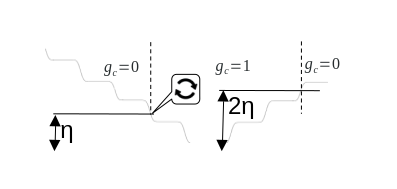
\includegraphics[width=0.5\textwidth,valign=c]{./task1b.png}
    \hfill \begin{minipage}{\dimexpr 0.5\linewidth-\columnsep}
        \caption{Representation of $g_c$ value at different level of energy with the indication of the direction change.}
        \label{task1b}
    \end{minipage}
\end{figure}
\end{description} 

\subsubsection{Task 2: Cued environment decision} \begin{description}
  \item[Strategy] Restrict navigation to the half-loop without a closed path, as indicated by a color that has already been seen once.
  \item[Heuristic] Detect and store the first color blob, and choose to turn in the direction it appears again. \\ The detection is reset when the energy decreases.
    \item[Internal variable] \eqline{\begin{array}{lll}
        c_{c\bullet} \in \{0, 1\} , \bullet \in \{b_{\mbox{blue}}, r_{\mbox{red}}\} & \left. c_{p\bullet} i \right|_{t = 0} = 0 & \mbox{Detected the color cue code, if any.} \\
    \end{array}}
    \item[Programmatoid solution] \eqline{\begin{array}{rcl}
        \multicolumn{3}{l}{\mbox{Detect the cue, if not yet done, and reset below an energy threshold}} \\
        c_{cb} &\leftarrow& \mbox{if }  c_{cb} = 0 \mbox{ and } c_{cr} = 0 \mbox{ and } (c_{lb} = 1 \mbox{ or } c_{rb} = 1) \mbox{ then} 1 \mbox{ elif } g_e < \eta/2 \mbox{ then } 0 \mbox{ else } c_{cb} \\
        c_{cr} &\leftarrow& \mbox{if }  c_{cb} = 0 \mbox{ and } c_{cr} = 0 \mbox{ and } (c_{lr} = 1 \mbox{ or } c_{rr} = 1) \mbox{ then} 1 \mbox{ elif } g_e < \eta/2 \mbox{ then } 0 \mbox{ else }c_{cr} \\
        \multicolumn{3}{l}{\mbox{Set the direction according to the cue}} \\
        q_p &\leftarrow& \mbox{if }  c_{lb} = c_{cb} \mbox{ or }  c_{lr} = c_{cr} \mbox{ then } 0 \mbox{ elif } c_{rb} = c_{cb} \mbox{ or }  c_{rr} = c_{cr} \mbox{ then } 1 \mbox{ else } q_p \\
   \end{array}} \end{description}

\subsubsection{Task 3: Valued environment decision} \begin{description}
   \item[Strategy and Heuristic] Test energy sources and change direction if the latter yields less increase than the former.
   \item[Internal Variables] \eqline{\begin{array}{lll}
     g_{c\flat} \in [0, 1], \flat \in \{1, 2\} &\left.g_{c\flat} \right|_{t = 0} = 0 & \mbox{Last and last-before-last cumulative energy increases.}\\
     g_{e\flat} \in [0, 1], \flat \in \{1, 2\} &\left.g_{e\flat} \right|_{t = 0} = 0 & \mbox{Last and last-before-last energy value.} \\
    \multicolumn{2}{l}{b_{di} \defq g_{e} > g_{e1}  \mbox{ and } g_{e1} < g_{e2}} & \mbox{Increase starts,  after a decrease.} \\
    \multicolumn{2}{l}{b_{ii} \defq g_{e} > g_{e1}  \mbox{ and } g_{e1} > g_{e2}} & \mbox{Increase continues.} \\
    \multicolumn{2}{l}{b_{id} \defq g_{e} < g_{e1}  \mbox{ and } g_{e1} > g_{e2}} & \mbox{Increase has just stopped, now decreases.} \\
    \multicolumn{2}{l}{b_{i} \defq g_{c2} > g_{c1}} & \mbox{Previous energy increase is higher.} \\
   \end{array}}
  \item[Programmatoid solution] \eqline{\begin{array}{rcl}
      q_p &\leftarrow& \mbox{if } b_{id} \mbox{ and }  b_{i} \mbox{ then } 1 - q_p \mbox{ else } q_p \\
   \multicolumn{3}{l}{\mbox{Then, in sequence:}} \\
     g_{c2} &\leftarrow& \mbox{ if } b_{di}  \mbox{ then } g_{c1} \mbox{ else } g_{c2} \\
     g_{c1} &\leftarrow& \mbox{ if } b_{di}  \mbox{ then } g_{e} - g_{e1} \mbox{ elif } b_{ii} \mbox{ then } g_{c1} + (g_{e} - g_{e1}) \mbox{ else } g_{c1} \\
     g_{e2} &\leftarrow& g_{e1} \\
     g_{e1} &\leftarrow& g_{e} \\
  \end{array}}
    It is important to note that evaluation is to be done in sequence, for the mechanism to be valid.
\begin{figure}[H]
  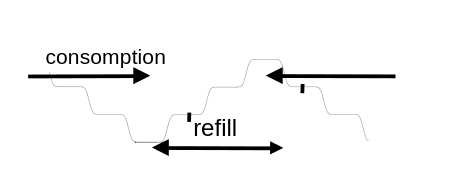
\includegraphics[width=0.5\textwidth,valign=c]{./energy-step.png}
    \hfill \begin{minipage}{\dimexpr 0.5\linewidth-\columnsep}
        \caption{Representation of energy profile when cumulative energy increase starts (first tick), with $g_{e} > g_{e1}  < g_{e2}$, and stops (last tick), with $g_{e} < g_{e1}$, while during refill $g_{e} > g_{e1}  > g_{e2}$.}
        \label{energy-step}
    \end{minipage}
\end{figure}
\end{description}

\section{Programmatoid computation} \label{programmatoid}

\subsection{Definition of a programmatoid computation}

We name ``programmatoid computation'' the conception of an input-output \href{https://en.wikipedia.org/wiki/Straight-line_program}{straight-line program} implementing an operator on either binary values $\in \{0, 1\}$ or continuous normalized\footnote{An alternative would have be to consider continuous normalized values $\in [-1, 1]$, with the sign function, and its mollification using $\mbox{tanh}(\cdot)$:
\eqline{\mbox{Sg}(x) \defq \mbox{if } x > 0 \mbox{ then } 1 \mbox{ elif } x < 0 \mbox{ then } -1 \mbox{ else } 0 = -1 + 2 \, \mbox{H}(x) = \lim_{\omega \rightarrow +\infty} \mbox{tanh}(\omega \, x),}
which would have yields to same general results, with somehow heavier derivations, as the reader can verify.

Implementing signed variable is obvious in a programmatoid environment:
\eqline{s = s_+ - s_-, \left\{\begin{array}{rcl} s_+ &\defq& \mbox{if } s  > 0 \mbox{ then } s \mbox{ else } 0 \\ s_- &\defq& \mbox{if } s  < 0 \mbox{ then } -s \mbox{ else } 0, \\ \end{array} \right.}
thus manipulating signed variables in a environment with only positive variables.} values $\in [0, 1]$, which evolution is defined using an LN-system with linear units or the step-function $\mbox{H}(\cdot)$ as non-linearity, this writing:
\eqline{o_n[t] = \left\{ \begin{array}{r} \mbox{H}(z_n[t]) \\ \mbox{Id}(z_n[t]) \\ \end{array} \right., z_n[t] \defq \sum_{m\in\{1,M\}} w_{nm} \, i_m[t-1] + w_{n0}, n \in \{1, N\}}
where $\mbox{Id}(\cdot)$ stands for the identity function. Here
\\\tab - $i_m[t]$ is the $m$-th input at a discrete $t$, $\left. i_m[t] \right|_{t=0} = 0$and
\\\tab - $o_n[t]$ is the $n$-th output a time $t$
\\ including recurrent system with some output corresponding to inputs, while
\\\tab - $w_{nm}, n \in \{1, N\}, m \in \{ 0, M \}$ are the systems parameters, or, weights for $m > 0$ and bias for $m = 0$.

By design, evaluation is done in sequence at a given $t$, i.e., from $o_1[t]$ to $o_N[t] $.

The step-function, also called Heaviside function, implements the computation of the sign of a value:
\eqline{\begin{array}{rcl}
    \mbox{H}(x) &\defq& \left\{ \begin{array}{rcl} 1 &\mbox{if}& x > 0\\ 1/2 &\mbox{if}& x = 0\\ 0 &\mbox{if}& x < 0\\ \end{array}\right. \\
    &=& \mbox{if } x > 0 \mbox{ then } 1 \mbox{ elif } x = 0 \mbox{ then } 1/2 \mbox{ else } 0. \\
\end{array}}
The design choice of $\mbox{H}(0) = 1/2$, instead for instance $\mbox{H}(0)=0$, this latter simplifying some formula, is due the neuronoid approximation developed in the sequel.

By extension, we use,  for any property ${\cal P}$, the notation:
\eqline{\mbox{H}({\cal P}) \defq \mbox{if } {\cal P} \mbox{ then } 1 \mbox{ else } 0}

A ``generalized programmatoid computation'' may include other dedicated non-linearities, providing these are \href{https://en.wikipedia.org/wiki/Pure_function}{pure fonction}, i.e., no side effect, same inpouts yield same output, and providing execution time does not depends on the input, while reasonably small; this will not used here.

For the sake of simplicity if the left hand size correspond to a value at time $t$ and right-hand size to values at $t-1$, which will be always here, and if not informative, temporal indexes are omitted, i.e. the previous equation will be written: 
\eqline{o_n  \leftarrow \mbox{H}(\sum_{m\in\{1,M\}} w_{nm} \, i_m + w_{n0}), n \in \{1, N\}}

\subsection{Comparison implementation}

Given two numerical variables $v_1$ and $v_2$, using the notation ,
we have the equivalence\footnote{
Considering the pseudo truth table, with $\mbox{H}(0) = 1/2$:
\eqline{\begin{array}{c|c|c|l|}
                                                             &\mbox{H}(v_1 > v_2) &\mbox{H}(v_1 = v_2) & \mbox{H}(v_1 < v_2) \\\hline
    \mbox{H}(v_1 - v_2)                                      & 1                  &   1/2           & 0 \\
    \mbox{H}(\mbox{H}(v_1 - v_2))                                 & 1                 &   1              & 0 \\
    \mbox{H}(\mbox{H}(v_2 - v_1))                                 & 0                 &   1              & 1 \\
    \mbox{H}(\mbox{H}(v_1 - v_2)) +\mbox{H}(\mbox{H}(v_2 - v_1))-1   & 0                 &   1              & 0 \\ \hline
\end{array}}  we obtain the expected results.}, considering $true$ as $1$ and $false$ as $0$:
\eqline{\begin{array}{|c|c|c|c|l}
    \mbox{H}(v_1 > v_2)                            & \mbox{H}(v_1 \le v_2)                        & \mbox{H}(v_1 = v_2)                                                    & \mbox{H}(v_1 \ne v_2)         \\  \hline
    \mbox{ not } \mbox{H}(v_1 \le v_2)   & \mbox{H}(\mbox{H}(v_1 - v_2))                      & \mbox{H}(v_1 \le v_2)  \mbox{ and } \mbox{H}(v_2 \le v_1)   & \mbox{ not } \mbox{H}(v_1 = v_2)                  & \mbox{with } \mbox{H}(0) = 1/2\\ \hline
    \mbox{H}(v_1 - v_2)                            & \mbox{ not } \mbox{H}(v_1 - v_2)     & \mbox{ not } \mbox{H}(v_1 \ne v_2)                          &\mbox{H}(v_1 > v_2) \mbox{ or } \mbox{H}(v_2> v_1)  & \mbox{with } \mbox{H}(0) = 0\\
\hline\end{array}}
while $\mbox{H}(v_1 < v_2) = \mbox{H}(v_2 > v_1)$ and $\mbox{H}(v_1 \ge v_2) = \mbox{H}(v_2 \le v_1)$. We thus can implement any numerical comparison as a programmatoid, providing that we can implement boolean expressions, as given now.

\subsection{Boolean expression implementation}

Given binary variables $b_n \in \{0_{{false}}, 1_{{true}}\}, n \in \{1, N\}$ we have the obvious\footnote{Easy to verify with, e..g., a truth table, and by induction for the generalized formula.} correspondence:
\eqline{\begin{array}{|c|c|c|c|} \hline
    b_1               & b_1 \mbox{ and } b_2                &  b_1 \mbox{ or } b_2   & \mbox{ not } b_1 \\ \hline
    \mbox{H}(b_1 - 1/2) & b_1 \, b_2 = \mbox{H}(b_1 + b_ 2 - 3/2)  & \mbox{H}(b_1 + b_ 2 - 1/2)       & 1 - b_1  = \mbox{H}(1/2 - b_1) \\ \hline
\end{array}} and more generally:
\eqline{\begin{array}{rcl}
    \mbox{and}_{n \in \{1, N\}} &=& \mbox{H}\left(\sum_{n \in \{1, N\}} b_n - N + 1/2\right) = \prod_{n \in \{1,  N\}} \mbox{H}(b_n - 1/2) = \prod_{n \in \{1,  N\}} b_n \\
    \mbox{or}_{n \in \{1, N\}} &=& \mbox{H}\left(\sum_{n \in \{1, N\}} b_n - 1/2\right) \\
\end{array}}

An interesting consequence is that binary variable products can be translated to a programmatoid.

Let us also notice that all arguments $x$ of the step function $\mbox{H}(\cdot)$ still verify $|x| \ge 1/2$.

\subsection{Conditional expression implementation}

A conditional expression on variables on any numerical type $v_n, n \in \{0, 1\}$  with a binary variable $b_1 \in \{0, 1\}$ writes: \eqline{\begin{array}{rcl}
     v &\leftarrow& \mbox{if } b_1 \mbox{ then } v_1 \mbox{ else } v_0 \\
    &=& b_1 \, v_1 + (1 - b_1) \, v_0 \\
    \multicolumn{3}{l}{\mbox{while, for binary variable, i.e., if and only if $v_n \in \{0, 1\},  n \in \{0, 1\}$: }} \\
    &=& \mbox{H}(v_1 + b_1 - 3/2) + \mbox{H}(v_0 + (1 - b_1) - 3/2) \\
    &=& \mbox{H}(v_1 + b_1 - 3/2) + \mbox{H}(v_0 - b_1 - 1/2) \\
    &=& \mbox{H}(\mbox{H}(v_1 + b_1 - 3/2) + \mbox{H}(v_0 - b_1 - 1/2)) \\
\end{array}}
as easy to verify, using for instance a truth table. Here:
\\- products with $(1 - b_1)$ and $b_1$ behaves as switches between $v_o$ and $v_1$
\\ - when $v_i$ are binary, we are left with a two layer computation, the first layer being built from two programmatoid,
and the second layer from either another programmatoid or a simple linear unit, i.e., a linear combination of values.
        
This generalizes to conditional expressions on variables on any numerical type $v_n, n \in \{0, N\}$: \footnote{
By induction, considering the second line, one one hand, due to the products, if $b_n = 0, n \in \{1, N\}$ we obtain $v_0$.
On the other hand, if $b_k = 0, k < K$ and $b_K = 1$, due the products, we obtain $v_K$, which is precisely the semantic
of the conditional expression of the first line. \\
The 3rd line is deduced from the second line, transforming the binary products on the corresponding programmatoid while:
\eqline{\begin{array}{rcl}
    h_0 &\defq& \mbox{H}(\sum_{n' \in \{1,  N\}} (1 - b_{n'}) - N + 1/2) \\ &=& \mbox{H}(1/2 - \sum_{n' \in \{1,  N\}} b_{n'})\\
    h_n &\defq& \mbox{H}(b_n + \sum_{n' \in \{1,  N\}, n' \ne n} (1 - b_{n'})  - N + 1/2) \\ &=& \mbox{H}(b_n - \sum_{n' \in \{1,  N\}, n' \ne n} b_{n'} - 1/2) \\
\end{array}}
The 4rd line integrates the $v_n$ variables in the programmatoid sum, since they are binary,
and provides the same obvious algebraic reduction as for the 3rd line.}: \eqline{\begin{array}{rcl}
v &\leftarrow& \mbox{if } b_1 \mbox{ then } v_1 \left[ \mbox{ elif } b_n \mbox{ then } v_n \right]_{n \in \{2, N\}} \mbox{ else } v_0 \\
    &=& \prod_{n' \in \{1,  N\}} (1 - b_{n'}) \, v_0  \\&+& \sum_{n \in \{1, N\}} \, b_n \, \prod_{\small \begin{array}{c}n' \in \{1,  N\}, \\ n' \ne n \\ \end{array}} (1 - b_{n'})  \, v_n  \\
   &=& \sum_{n \in \{0, N\}} h_n \, v_n \\
\mbox{ with } h_0 &\defq& \mbox{H}(1/2 - \sum_{n' \in \{1,  N\}} b_{n'})  \in \{0, 1\}\\
\mbox{ and } h_n &\defq&  \mbox{H}(b_n - \sum_{n' \in \{1,  N\}, n' \ne n} b_{n'} - 1/2) \in \{0, 1\}, n \in \{1, N\} \\
    &&\\ \multicolumn{3}{l}{\mbox{while, for binary variable, i.e., if and only if $v_n \in \{0, 1\},  n \in \{0, N\}$: }} \\
    &=& \mbox{H}(v_0 - \sum_{n' \in \{1,  N\}} b_{n'} - 1/2)  \\ &+& \sum_{n \in \{1, N\}} \mbox{H}(v_n + b_n - \sum_{n' \in \{1,  N\}, n' \ne n} b_{n'} - 3/2). \\
\end{array}}

Let us also notice that all arguments $x$ of the step function $\mbox{H}(\cdot)$ again verify $|x| \ge 1/2$.

\begin{quotation}
As a consequence,
\\\tab - {\em A $N$-term conditional expression on binary variables reduces to a two layers programmatoid of $N$ and $1$ unit, the former unit being either linear of with a step-wise function.}
\\ \tab - {\em A $N$-term conditional expression on continuous variables reduces to a  two layers system of $N$ programmatoid and an output unit with $h_n$ exclusive switches, as defined in the sequel.}
\end{quotation}
  
\section{Neuronoid computation} \label{neuronoid}

\subsection{Neuronoid unit}

By ``neuronoid'' we name the \href{https://en.wikipedia.org/wiki/Biological_neuron_model#Relation_between_artificial_and_biological_neuron_models}{not very biologically plausible} simplest biological neuron or neuron small ensemble inspired by \href{https://inria.hal.science/cel-01095603v1}{mean-field modeling} of the \href{https://en.wikipedia.org/wiki/Hodgkin-Huxley_model}{Hodgkin–Huxley neuronal axon model}.

It is defined the equation:
\eqline{\begin{array}{rcll}
  \multicolumn{4}{l}{\tau \frac{\partial v_i}{\partial t}(t) + v_i(t) = z_i(t), \;\;\;z_i(t) \defq \mbox{h}\left(\sum_j \, w_{ij} \, v_j(t) + w_{i0}\right),} \\ \\
  \mbox{h}(x) &\defq& 1/\left(1+e^{-4\,x}\right) \\
         &=& (1+ \mbox{tanh}(2 \, x)) / 2 = \mbox{sech}(2 \, x) \, e^{2 \, x} /2 & \mbox{(tanh linear relation)}\\
         &=& \mbox{h}(x_0) + \mbox{sech}(2 \, x_0)^2 \, (x - x_0) + O((x - x_0)^2), & \mbox{(local 1st order behavior)}\\
         &=& 1 - e^{-4 \,x} + O(e^{-8 \, x)}) & \mbox{(behavior toward infinity).}\\
\end{array}}
Here,  $\mbox{h}(\cdot)$ is the normalized sigmoid with: \eqline{\mbox{h}(-\infty) = 0, \mbox{h}(0) = 1/2, h'(0) = 1, \mbox{h}(+\infty) = 1, \mbox{h}(x) = 1 - \mbox{h}(-x),} and is derived from from considerations on mean-field modeling \cite{cessac_neuron_2007}.

Following this weak analogy with biological neurons, $v_i$ stands for the membrane potential, so that:
\eqline{\begin{array}{rcll} v(t)
  &=& 1/\tau \, \int_0^t e^{-(t-s)/\tau} \, z(s) \, ds + v(0) \, e^{-t/\tau} \\
  &=& \left. z(0) + e^{-t/\tau} \, (v(0) - z(0)) \right|_{z(t)= z(0)} & \mbox{ (constant input)}\\
   &=& \left. z(t) \right|_{\tau = 0} & \mbox{ (no leak),}\\
  \multicolumn{4}{l}{\mbox{and the corresponding discrete approximation using an Euler schema writes:}} \\
  &\simeq&  (1-\gamma) \, v(t-\Delta t) + \gamma \, z(t-\Delta t)) \\
  &=& \sum_{s=0}^{t-1} \gamma \, (1-\gamma)^{t-s+1} \, z(s) + v(0) \, (1-\gamma)^t \\
  &=& \left. z(0) + (1-\gamma)^t \, (v(0) - z(0)) \right|_{z(t)= z(0)} & \mbox{ (constant input)}\\
  &=& \left. z(t) \right|_{\gamma = 1} & \mbox{ (no leak)}. \\
\end{array}} 
with $0 < \gamma < 1$ and $0 < \tau$ in one-to-one correspondence:
\eqline{\gamma \defq 1 - e^{\frac{1}{\tau}} \Leftrightarrow \tau = -\frac{1}{\log\left(1-\gamma\right)},  \mbox{while} \lim_{\gamma \rightarrow 0} \tau = +\infty , \lim_{\gamma \rightarrow 1} \tau = 0.}

All this is just very standard derivations, available as \href{https://raw.githubusercontent.com/vthierry/braincraft/master/doc/tex/neuronoid.mpl.out.txt}{{\tt Maple} code}, of the vanilla neuron model, as already proposed by \cite{lapicque_recherches_1907}.

The leak term, in the discrete case, is computationally equivalent to a recurrent linear connection: It will thus be implemented as such in the sequel.

\subsection{Definition of a neuronoid computation}

We call ``neuronoid computation'' the conception of an input-output transform based on feed-forward and recurrent combination with only neuronoids as non-linearities:
\eqline{o_n[t] = \mbox{h}(z_n[t]), z_n[t] \defq \sum_{m\in\{1,M\}} w_{nm} \, i_m[t-1] + w_{n0}, n \in \{1, N\}}
with the same notations as for programmatoid computations, and with determistic evaluation sequence.

\subsection{Step-function mollification}

The step-function approximates sigmoid with a huge slope at zero, i.e.:
\eqline{\forall x \ne 0, \mbox{H}(x) = \lim_{\omega  \rightarrow +\infty} \mbox{h}(\omega \, x), \left. h'(\omega \, x)  \right|_{x = 0} =  \omega}
while the convergence is also obtained for $v=0$ in the distribution sense with $\mbox{H}(0) = \mbox{h}(0) = 1/2$.
More precisely, the ${\cal L}_1$ error magnitude, on $]-\infty, +\infty[$, writes:
\eqline{|\epsilon_{H,\omega}(x) |_{{\cal L}_1} = \frac{\log(2)}{2} \, \frac{1}{\omega}, \epsilon_{H,\omega}(x) \defq \mbox{H}(x) - \mbox{h}(\omega \, x)}
while:
\eqline{|\epsilon_{H,\omega}(x)| = e^{-4\,\omega}+O\left(e^{-8\,\omega}\right)}

It has been noticed that, except for numerical comparisons, all arguments $x$ of the step function $\mbox{H}(\cdot)$ verify $|x| \ge 1/2$, and the related error is negligible as soon as, say, $\omega \ge 10$:
\eqline{\begin{array}{|l|c|c|c|c|c|c|} \hline
  \omega & 1 & 2 & 5 & 10 & 20 & 50 \\ \hline
  \epsilon_\omega(\pm1/2) & 0.119 &  0.0180 &  0.455 \, 10^{-4} &  0.206 \, 10^{-10} &  0.426 \, 10^{-19} &  0.372 \, 10^{-45} \\ \hline
\end{array}}

\begin{quotation}
- {\em Any programmatoid  computation involving the $\mbox{H}(\cdot)$ function can thus be approximated by a neuronoid, with $\tau = 0$, and sufficiently large $\omega$, with an exponentially decreasing residual.}
\end{quotation}
  
Derivations are available as \href{https://raw.githubusercontent.com/vthierry/braincraft/master/doc/tex/mollificatio.mpl.out.txt}{{\tt Maple} code}.

\subsection{Approximation of the identify function}

We also have to use a the linear part sigmoid to approximate the identity function $\mbox{Id}(x) = x$ defining:
\eqline{\begin{array}{rcl}
   \mbox{Id}_{\omega'}(x) &\defq& \omega' \, (\mbox{h}(x/\omega') - 1/2) \\
                           &=& x - \frac{4}{3} \frac{1}{\omega'^2} \, x^3 + O\left(x^5\right) \\
\end{array}} 
and writing $\epsilon_{l,\omega'}(x) \defq x - l_{\omega'}(x)$ , the ${\cal L}_1$ error magnitude on $[-M, +M]$ writes:
\eqline{\int_{x=-M}^{x=+M}|\epsilon_{l,\omega'}(x)| \, dx = \frac{2}{3} \, \frac{M^4}{\omega'^2} + O\left(\frac{1}{\omega'^4}\right)}
and the related ${\cal L}_0$ error magnitude:
\eqline{\max(|\epsilon_{l,\omega'}(x)|), x \in [-M, M] = \epsilon_{l,\omega'}(M)  = \frac{4}{3} \, \frac{M^3}{\omega'^2} + O\left(\frac{1}{\omega'^4}\right)}

In a positive interval, by symmetry, the ${\cal L}_1$ error magnitude is divided by $2$, while the ${\cal L}_0$ error magnitude is the same.

The identity function is thus impaired by a bias $\pm \frac{4}{3} \, \frac{M^3}{\omega'^2}$ reducing the output value with respect to the input value.

Assuming values are normalized, in the $[-1, +1]$ interval or in the $[0, 1]$ interval, we obtain, for the ${\cal L}_0$ error magnitude:
\eqline{\begin{array}{|l|c|c|c|c|c|c|} \hline
\omega' & 10 & 50 & 100 & 200 & 500 & 1000  \\ \hline
\epsilon_{l,\omega'}(1) & 0.0131 &  0.533 \, 10^{-3} &  0.133 \, 10^{-3} &  0.333 \, 10^{-4} &  0.54\, 10^{-7} &  0.12\, 10^{-7}  \\ \hline
\end{array}}
with a negligible error for, say, $\omega'  \ge 100$.

At the implementation level we must introduce a change of variable, and consider:
\eqline{\mbox{Jd}_{\omega'}(x)  \defq \mbox{h}(x/\omega') \\ \mbox{ with } \left\{\begin{array}{l} \mbox{Id}_{\omega'}(x) = \omega' \, (\mbox{Jd}_{\omega'}(x) - 1/2) \\ \mbox{Jd}_{\omega'}(x) = \mbox{Id}_{\omega'}(x) / \omega' + 1/2 \\ \end{array} \right.}
in order to define a proper neuronoid computation, in the form given as definition. It is obvious to propagate this change of variable in all the equations.

It must be noted that although continous variables stands in $[0, 1]$ because of negative weights in the linear combination of input, intermediate values may be negative, as considred here.

\begin{quotation}
- {\em Any programmatoid  computation involving the $\mbox{Id}(\cdot)$ function can thus be approximated by a neuronoid, with $\tau = 0$, up to an affine change of variable, and sufficiently large $\omega'$, and a residual decreasing in a square way.}
\end{quotation}
  
Derivations are available as \href{https://raw.githubusercontent.com/vthierry/braincraft/master/doc/tex/linearapproximation.mpl.out.txt}{{\tt Maple} code}.

\begin{quotation}
Collecting the previous results, we obtain:\\
- {\em Any programmatoid computation can be approximated, up to any precision, by a neuronoid computation.}
\end{quotation}

\subsection{Approximation of switch mechanisms}

Given normalized floating point variables $v_n \in [-1, 1], n \in \{1, N\}$ and binary variables $b_n \in \{0, 1\}, n \in \{1, N\}$, conditional expressions and related mechanisms require the implementation of formula of the form\footnote{We easily verifies that:
\\ - if $b_n= 0$, while $|v_n/\omega'| \le 1/\omega' \ll 1$, the term $\omega' \, \mbox{h}(v_n/\omega' + \omega \, b_n - \omega) \simeq \mbox{h}(- \omega) \simeq 0$ up to $O\left(e^{-4\,w}\right)$ as derived previously, while
\\ - if $b_n= 1$,the term $\omega' \, \mbox{h}(v_n/\omega' + \omega \, b_n - \omega) = \omega' \, \mbox{h}(v_n/\omega')$ corresponds to the approximation of the identity function, up to $O\left(\frac{1}{\omega'}\right)$ as derived previously.}:
\eqline{\begin{array}{rcl}
    v &=& \sum_{n \in \{0, N\}} b_n \, v_n \\
    &=& \sum_{n \in \{0, N\}} \omega' \, \mbox{h}(v_n/\omega' + \omega \, b_n - \omega) + O\left((\omega')^{-2}\right)+ O\left(e^{-4\,\omega}\right) \\
\end{array}}

The key point here is that product of a continuous variable $v_n$ by a binary variable $b_n$, acting as a kind of switch, is not implementable with pure programmatoid computation because only products with constant parametric values, or weights. Up to our best understanding product between two variables, one being continuous can not be defined with lineat combinations unless additional mechanisms are introduced, as discussed below.

We also notice that the $\mbox{Id}(\cdot)$ function mollification approximation is less efficient that the $\mbox{H}(\cdot)$ function mollification, the former being subject to a polynomial remainder, the latter to an exponential one.

\begin{quotation}
This means that:
\\\tab - {\em Neuronoid computation allows one to implement more mechanism approximations, that exact programmatoid computation only.}
\end{quotation}

\section{Examples of programmatoid computation}

A step ahead, t seems obvious that we can designed temporizing mechanisms, oscillators and sequence generator, sleep sort mechanism, etc.

\subsection{Memory gate}

For a data input $i$, a control $i_l \in \{0, 1\}$, and an output $o$, the equation:
\eqline{\begin{array}{rcl}
    o &\leftarrow& \mbox{if } i_l = 1 \mbox{ then } o \mbox{ else } i \\
\end{array}}
implements, if $i \in \{0, 1\}$, $o \in \{0, 1\}$, a 1 bit memory, i.e., also called a RS gate, and reusing the previous conditional instruction parameters.

The key point is that it is now a recurrent system, which stability is obvious at the programmatoid level,
but not necessarily at the neuronoid level, since we have an recurrent equation for $i_l = 1$.
\eqline{\begin{array}{rcl}
     \multicolumn{3}{l}{\mbox{For $i \in \{0, 1\}$, $o \in \{0, 1\}$ at the programmatoid level:}} \\
     o &\leftarrow& \mbox{H}(i - i_l - 1/2) + \mbox{H}(o + i_l - 3/2) \\
    &&\\\multicolumn{3}{l}{\mbox{For $i \in \{0, 1\}$, $o \in \{0, 1\}$:}} \\
     o &\leftarrow& \mbox{h}(\omega \, (i - i_l - 1/2) ) + \mbox{h}(\omega \, (o + i_l - 3/2)) \\
    &=& \left. O\left(e^{-4\,\omega}\right) + \mbox{h}(\omega \, (o  - 1/2)) \right|_{i_l = 1} \\
    &&\\\multicolumn{3}{l}{\mbox{For $i \in [-1, 1]$, $o \in [-1, 1]$:}} \\
    o &\leftarrow& \omega' \, (\mbox{h}(i/\omega' -  \omega \, i_l) + \mbox{h}(o /\omega' -  \omega \, (1 - i_l)) \\
    &=& \left. O\left(\omega' \, e^{-4\,\omega}\right) + \omega' \, \mbox{h}(o/\omega') \right|_{i_l = 1} \\
\end{array}}

\begin{itemize}
  \item The former equation is exact, so entirely stable during iterations.
 \item For the second equation, memorizing $\left.o\right|_{t=0} \in \{0, 1 \}$, thus with $i_l = 1$, for
\eqline{\epsilon \defq \left\{\begin{array}{cc} o &\left.\right|_{\left.o\right|_{t=0} = 0} \\ 1 - o&\left.\right|_{\left.o\right|_{t=0} = 1} \end{array} \right.}
we obtain\footnote{
For $\left.o\right|_{t=0} = 0$ the derivation is straightforward. For $\left.o\right|_{t=0} = 1$ and $i = 0$:
\eqline{\begin{array}{rcll}
    \epsilon
    &\leftarrow& 1 - o \\
    &=& 1 - \mbox{h}(-3/2 \, \omega) - \mbox{h}( \omega \, (1 - \epsilon + 1 - 3/2)) \\
    &=& 1 - \mbox{h}(-3/2 \, \omega) - \mbox{h}( \omega \, (-\epsilon + 1/2)) \\
    &=& - \mbox{h}(-3/2 \, \omega) + \mbox{h}(\omega \, (\epsilon - 1/2)) & \mbox{ since $\mbox{h}(x) = 1 - \mbox{h}(-x)$} \\
  \end{array}} with a similar derivation for $\left.o\right|_{t=0} = 1$ and $i = 1$.}:
\eqline{\begin{array}{rcl}
    \epsilon &\leftarrow& (1 - 2 \, \left.o\right|_{t=0}) \,  \mbox{h}(-(3/2 - i) \, \omega) + \mbox{h}( \omega \, (\epsilon - 1/2)) \\
    &=& \left\{\begin{array}{lrcll}
      0 &\epsilon&=& 0 & \mbox{ if $\left.o\right|_{t=0} = 1$}\\
      e^{-2 \, \omega} + O\left(e^{-4 \, \omega}\right) &\epsilon&=& \varepsilon \, e^{-2 \, \omega}& \mbox{otherwise}\\
   \end{array}\right. \\
\end{array}}
In words : the iteration remains stable, and the error at the order of magnitude of $O\left(e^{-2 \, \omega}\right)$. In particular the previous bias $\varepsilon$ only impacts the $O\left(e^{-4 \, \omega}\right)$ terms. Furthermore, if $\left.o\right|_{t=0} = 1$, the positive bias yields a convergence towards $1$ without any bias if $i = 1$, and with a exponentially decreasing bias if 
$i = 0$.

\item For the third equation, memorizing $\left.o\right|_{t=0} \in [-1, 1]$, thus with $i_l = 1$, while $i  \in [-1, 1]$, we obtain:
\eqline{\begin{array}{rcl}
    o &\leftarrow& \omega' \, (\mbox{h}(i/\omega' -  \omega \, i_l) + \mbox{h}(o /\omega' -  \omega \, (1 - i_l)) \\
    \multicolumn{3}{l}{\mbox{while, since $i_l = 1$:}} \\
    &=& \omega' \, (\mbox{h}(i/\omega' -  \omega) + \mbox{h}(o /\omega') \\
    \multicolumn{3}{l}{\mbox{while, when neglecting $|i/\omega'| < 1/\omega' \ll \omega$:}} \\
    &=& \omega' \, (\mbox{h}(-\omega) + \mbox{h}(o /\omega') \\
    \multicolumn{3}{l}{\mbox{while, using previous series formula:}} \\
    &=& o \pm \frac{4}{3} \, \frac{1}{\omega'^2} + e^{-4 \omega} + O\left(\frac{1}{\omega'^4}\right) + O\left(e^{-8 \omega}\right) \\
     \multicolumn{3}{l}{\mbox{while, considering only the larger term:}} \\
    &\simeq& o \pm \frac{4}{3} \, \frac{1}{\omega'^2}  = \left.o\right|_{t=0} \pm t \, \frac{4}{3} \, \frac{1}{\omega'^2} \\
 \end{array}}
The memorization is thus impaired by a linear bias only, thanks to the fact that linear unit has been normalized. Because $O\left(e^{-4 \omega}\right) \ll O\left(\frac{1}{\omega'^2}\right)$, fro the chosen values, the bias due the use of a neuronoid approximation of a programmatoid is negligible with respect to the bias due to the use of a neuronoid approximation of a linear unit.
\end{itemize}

Derivations are available as \href{https://raw.githubusercontent.com/vthierry/braincraft/master/doc/tex/memorygate.mpl.out.txt}{{\tt Maple} code}.

\subsection{Multi-stable mechanisms}

The previous developments leads to solutions for several temporal systems, as briefly given now.

\subsubsection{Bi-stable mechanisms}

\begin{figure}[H]
   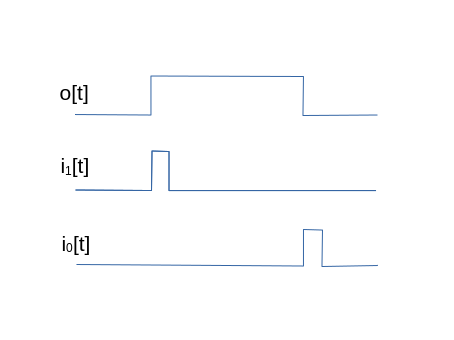
\includegraphics[width=0.5\textwidth,valign=c]{./bistable2.png}
    \hfill \begin{minipage}{\dimexpr 0.5\linewidth-\columnsep}
      \caption{With: \eqline{\begin{array}{rcl}
             o &\leftarrow& \mbox{ if } o = 0 \mbox{ and } i_1 = 1 \mbox{ then } 1 \\&& \mbox{ elif } o = 1 \mbox{ and } i_0 = 1 \mbox{ then } 0 \\&& \mbox{ else } o \\
         \end{array}}
        a bi-stable system with two $1$ and $0$ inputs, is implemented.
        }
        \label{bistable2}
    \end{minipage}
\end{figure}

\begin{figure}[H]
   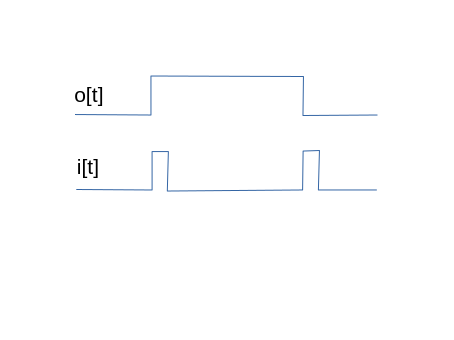
\includegraphics[width=0.5\textwidth,valign=c]{./bistable1.png}
    \hfill \begin{minipage}{\dimexpr 0.5\linewidth-\columnsep}
      \caption{With: \eqline{\begin{array}{rcl}
             o &\leftarrow& \mbox{ if } o = 0 \mbox{ and } i_1 = 1 \mbox{ then } 1 \\&& \mbox{ elif } o = 1 \mbox{ and } i_0 = 1 \mbox{ then } 0 \\&& \mbox{ else } o \\
             i_1 &\leftarrow& \mbox{ if } i_1 = 0 \mbox{ and } i = 1 \mbox{ then } 1 \\&& \mbox{ elif } o = 0 \mbox{ then } 0  \\&& \mbox{ else } i_1 \\
             i_0 &\leftarrow& \mbox{ if } i_0 = 0 \mbox{ and } i = 0 \mbox{ then } 1 \\&& \mbox{ elif } o = 1 \mbox{ then } 0  \\&& \mbox{ else } i_0 \\
         \end{array}}
         a bi-stable system with one two-way switch is implemented, using internal variables $i_0$ and $i_1$. This corresponds to a frequency divider by 2.
        }
        \label{bistable1}
    \end{minipage}
\end{figure}

\subsubsection{Spike generation}

\begin{figure}[H]
   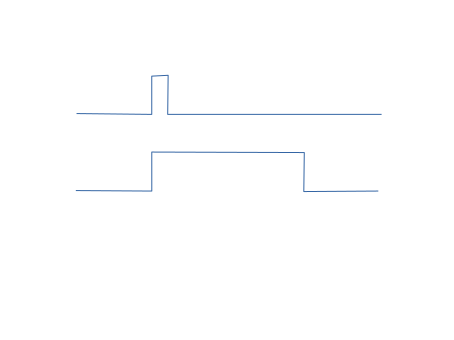
\includegraphics[width=0.5\textwidth,valign=c]{./spike1.png}
    \hfill \begin{minipage}{\dimexpr 0.5\linewidth-\columnsep}
      \caption{With: \eqline{\begin{array}{rcl}
             o &\leftarrow& \mbox{ if } r = 0 \mbox{ and } i = 1 \mbox{ then } 1 \\&& \mbox{ else } 0 \\
             r &\leftarrow& \mbox{ if } o = 1 \mbox{ then } 1 \\&& \mbox{ elif } i = 0 \mbox{ then } 0  \\&& \mbox{ else } r \\
         \end{array}}
         a spike generation detecting signal rising, with an internal variable $r$ registering if already detected.}
        \label{spike1}
    \end{minipage}
\end{figure}

\subsubsection{Delay}

\begin{figure}[H]
   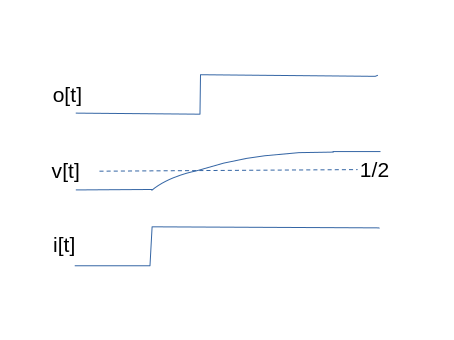
\includegraphics[width=0.5\textwidth,valign=c]{./delay1.png}
    \hfill \begin{minipage}{\dimexpr 0.5\linewidth-\columnsep}
      \caption{With: \eqline{\begin{array}{rcl}
             o &\leftarrow& \mbox{ if } v > 1/2 \mbox{ then } 1 \mbox{ else } 0 \\
             v &\leftarrow& (1-\gamma) \, v + \gamma \, i \\ 
         \end{array}}
        a delayed output is implemented. Assuming that $v = 0$, when $i=1$ and remains at this value, we obtain for the delay $T$:
        \eqline{T = -\frac{\log(2)}{\log(1 - \gamma)} > 0 \Leftrightarrow \gamma =  1 - 2^{-\frac{1}{T}}.}
        Here we assume that $i = 1, t \in [0, T]$ but it is very easy to avoid this constraint with a bi-stable mechanism as input.}
        \label{delay1}
    \end{minipage}
\end{figure}

Derivations are available as \href{https://raw.githubusercontent.com/vthierry/braincraft/master/doc/tex/delayastable.mpl.out.txt}{{\tt Maple} code}.

\subsubsection{Oscillation}

\begin{figure}[H]
   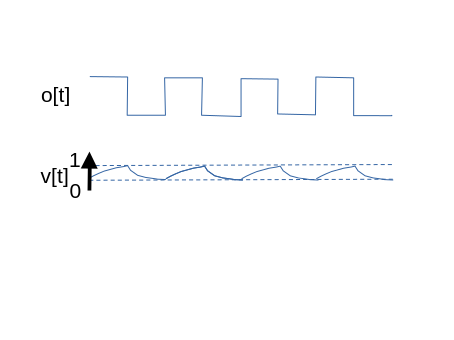
\includegraphics[width=0.5\textwidth,valign=c]{./astable1.png}
    \hfill \begin{minipage}{\dimexpr 0.5\linewidth-\columnsep}
      \caption{With: \eqline{\begin{array}{rcl}
             o &\leftarrow& \mbox{ if } v < 1/3 \mbox{ then } 0 \\&& \mbox{ elif } v > 2/3 \mbox{ then } 1 \\&& \mbox{ else } o \\
             v &\leftarrow& (1-\gamma) \, v + \gamma \, (1 - o) \, i \\ 
         \end{array}}
        an binary oscillator is implemented. It is stopped if $i=0$ and running for $i = 1$. We obtain for the period $T$:
        \eqline{T = -\frac{2 \, \log(2)}{\log(1 - \gamma)} > 0 \Leftrightarrow \gamma =  2 - 2^{1-\frac{1}{T}}.}}
        \label{astable1}
    \end{minipage}
\end{figure}

Derivations are available as \href{https://raw.githubusercontent.com/vthierry/braincraft/master/doc/tex/delayastable.mpl.out.txt}{{\tt Maple} code}.

\section{Examples of neuronoid computation} \label{softmax}

\subsection{The explog function} \label{explog}

The maximal and the average operators can be easily combined. For instance, given $K$ inputs $i_k \in [-1, 1], k \in \{1, K\}$, let us define:\eqline{\begin{array}{rcll}
    o &\defq& \frac{1}{\mu} \, \log\left(\frac{1}{K} \, \sum_{k \in \{1\cdots K\}}  \, \exp(\mu \, i_k)\right) \\
      &=& \frac{1}{K} \sum_k i_k + O(\mu) & \mbox{(average)} \\
    &=& \max_k(i_k) - \frac{\log(K)}{\mu} + \frac{O\left(e^{-\nu\,\mu}\right)}{\mu}, \nu > 0 & \mbox{(max)} \\
    &=& \left.i_1\right|_{i_i = i_2 \cdots = i_K} \\
    &\in& [-1, 1]\\
\end{array}}
with  $\mu > 0$ parameterizing the balance between:
\\\tab - the average, for small $\mu$, line 2 above,
\\\tab - the maximum, for large $\mu$, line 3 above, up to an offset $-\log(K)/\mu$,
\\ as shown in Figure~\ref{explog}.
\begin{figure}[H]
   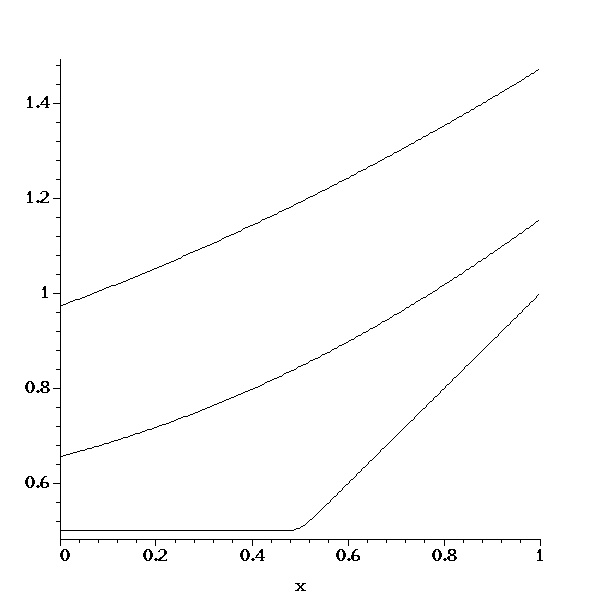
\includegraphics[width=0.5\textwidth,valign=c]{./explog.jpg}
    \hfill \begin{minipage}{\dimexpr 0.5\linewidth-\columnsep}
        \caption{Representation of the exp-log function for $K = 2$, $i_2 = 1/2$, with $i_1 \in [0, 1]$ and $\mu \in \{0.01, 0.1, 1, 10, 100\}$, from top to bottom, in black, orange, red, green and blue, respectively. With small $\mu$ it is closed to linear average, whereas for $\mu =100$ it is close to $\max(x, 1/2)$.}
        \label{explog}
    \end{minipage}
\end{figure}

From Figure~\ref{explog}, we observe that for $i_k \in [-1, 1]$, $\mu \in [0.01, 100]$ is a reasonable range to approximate the different profiles, so that:
\\\tab - The $\exp(\cdot)$ function range is in $[-100, 100]$.
\\\tab - The $\log(\cdot)$ function range is in $[e^{-100} \simeq 1, e^{100}]$.
\\ These are huge ranges but we may consider the following renormalization:\eqline{\begin{array}{rcll}
    i_k &\rightarrow& \frac{i_k}{\mu} \\ 
    o  &\rightarrow& \frac{o}{\mu} \\ 
   o &=& \log\left(\frac{1}{K} \, \sum_{k \in \{1\cdots K\}}  \, \exp(i_k)\right) \\
\end{array}}
so that the $\exp(\cdot)$ range is now $[-1, 1]$ and the $\log(\cdot)$ range is now $[1, e]$, allowing an implementation with not so big function's range. This is fine, providing that we can implement the $\exp(\cdot)$ and the $\log(\cdot)$ functions with a sufficient numerical precision, because, we now are working with small values of $i_k$.

Derivations of this section are available as \href{https://raw.githubusercontent.com/vthierry/braincraft/master/doc/tex/explog.mpl.out.txt}{{\tt Maple} code}.

\subsection{Approximation of {\tt exp} and {\tt log}}

Taking benefit of the fact that sigmoid is convex as the exponential function in some range, and concave as the logarithm function in some range, we can easily design the following approximations, obtained by some manual intuitive choice of the sigmoid combination and numerical adjustment of the parameters. Two examples are given in Figure~\ref{expneuronoid} and Figure~\ref{logneuronoid}. We share these examples to illustrate fact we really can approximate several bounded non-linear function with neuronoid, but we will use another track, to 

\begin{figure}[H]
  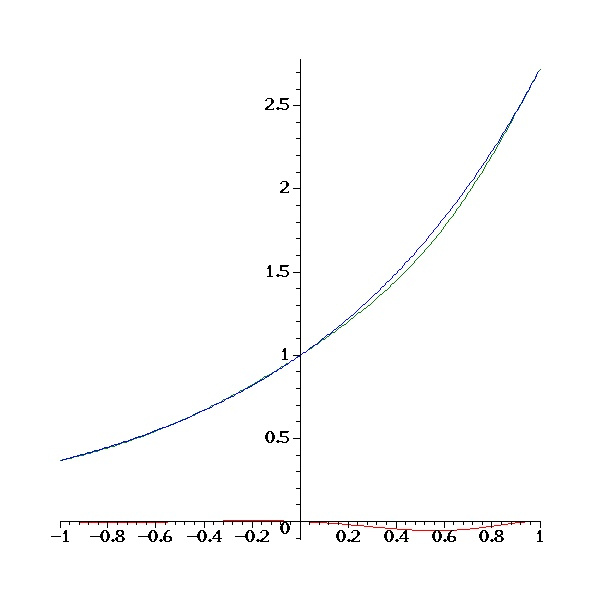
\includegraphics[width=0.5\textwidth,valign=c]{./expneuronoid.jpg}
    \hfill \begin{minipage}{\dimexpr 0.5\linewidth-\columnsep}
      \caption{Approximation in the $[-1, 1]$ interval of the exponential function, in blue, by a sigmoid combination, in green: \eqline{0.182 + 2.34 \,\mbox{h}(x - 1) + 1.55 \, \mbox{h}(x/2): } yielding a ${\cal L}_1$ error of $0.01$, the error being drawn in red.}
        \label{expneuronoid}
    \end{minipage}
\end{figure}

\begin{figure}[H]
  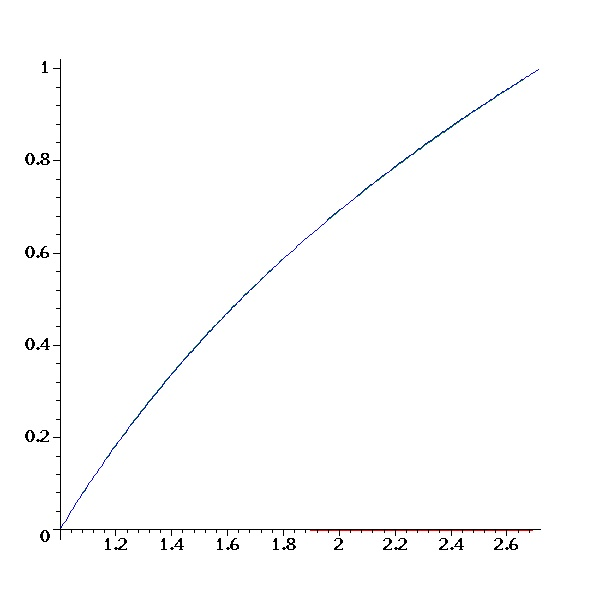
\includegraphics[width=0.5\textwidth,valign=c]{./logneuronoid.jpg}
    \hfill \begin{minipage}{\dimexpr 0.5\linewidth-\columnsep}
      \caption{Approximation in the $[1, e]$ interval of the logarithm $\log(x)$ function, in blue, by a sigmoid combination, in green: \eqline{-5.10 + 2.60 \,\mbox{h}(x/2) + 4.70 \, \mbox{h}(x/10): } yielding a ${\cal L}_1$ error of $0.001$, the error being drawn in red.}
        \label{logneuronoid}
    \end{minipage}
\end{figure}

Given these two approximations, we can implement an approximation of the renormalized {\tt explog} function proposed previously, with $N_l = 1$ in this case.

Derivations of this section are available as \href{https://raw.githubusercontent.com/vthierry/braincraft/master/doc/tex/explog.mpl.out.txt}{{\tt Maple} code}.

\subsection{Approximation of valued product.}

Let us now consider two values $v_i \in [-1, 1], i \in \{1, 2\}$, and apply the basic formula:
\eqline{\exp(\log(v_1)+\log(v_2)) = v_1 \, v_2}
in such a way that the the $\log()$ and $\exp()$ functions are used within the ranges defined previously. We obtain:

\eqline{\begin{array}{rclcl}
    l(v_i) &\defq& \frac{e-1}{2} \, v_i + \frac{e+1}{2} &\in& [1_{v_i = -1}, e_{v_i = 1}], \\
    l(v_1, v_2) &\defq& \log(l(v_1)) + \log(l(v_2)) -1 &\in& [-1, 1] , \\
    b &\defq& \frac{4}{(e -1)^2}  &c& \defq \mbox{coth}\left(\frac{1}{2}\right) \\
    p(v_1, v_2) &\defq& b \, e^{l(v_1, v_2)} - c \, (v_1 + v_2 + c) \\
    &=& v_1 \, v_2
\end{array}}

Therefore,  valued products can be approximated by neuronoids. This for instance quite useful for mechanism of gain control or using adaptive mechanisms, as for instance a softmax mechanism discussed now.
    
Derivations of this section are available as \href{https://raw.githubusercontent.com/vthierry/braincraft/master/doc/tex/explog.mpl.out.txt}{{\tt Maple} code}.

\subsection{Approximation a softmax operator}

Another track is to consider the programmatoid implementation of the maximum operator, given $K$ inputs $i_k \in [-1, 1], k \in \{1, K\}$, as a weighted sum:
\eqline{o \defq \max_k(i_k) = \sum_k b_k \, i_k}
with:
\eqline{b_k \defq And_{l \in \{1, k-1\}} \mbox{H}(i_k >  i_l) \mbox{ and } And_{l \in \{k+1, K\}} \mbox{H}(i_k \ge i_l),}
So that $b_k = 1$ if $i_k$ is the first instantiating of the max value \footnote{
First, assume that all $i_k$ are different; then $b_k = 1$ if and only if $\forall l \ne k, i_k > i_l$, yielding the expected result.\\
Then, if more than one value corresponds to $\max_k(i_k)$, let us consider $k_0 = \mbox{ argmin} \{k, k = \max_k(i_k)\}$. \\
For $k_0$, $And_{l \in \{k_0+1, K\}} \mbox{H}(i_{k_0} \ge i_l) = 1$ because it is a maximum and $And_{l \in \{1, k_0-1\}} \mbox{H}(i_{k_0} >  i_l) =1$ because no previous maximum is encountered, by definition. Then for subsequent values $k_1 = \max_k(i_k)$, because there is $k_0 < k_1$ with $i_{k_0} = i_{k_1}$, then $And_{l \in \{1, k_1-1\}} \mbox{H}(i_{k_1} >  i_l) = 0$, so that we only have one occurrence of $i_k$ which is selected.}, thus with a form similar to the average operator $\mbox{mean}_k(i_k) = 1/K \, \sum_k b_k \, i_k$.

We easily derive:
\eqline{\begin{array}{rcl}
    b_k &\defq& And_{l \in \{1, k-1\}} \mbox{H}(i_k >  i_l) \mbox{ and } And_{l \in \{k+1, K\}} \mbox{H}(i_k \ge i_l) \\
    \multicolumn{3}{l}{\mbox{while, expanding the $And$ operator}}\\
    &=&  \mbox{H}\left(\sum_{l \in \{1, k-1\}}  \mbox{H}(i_k >  i_l) + \sum_{l \in \{k+1, K\}} \mbox{H}(i_k \ge i_l) - K + 3/2\right). \\
\end{array}}

Then, introducing a linearly combination of both operators:
\eqline{\begin{array}{rcl}
    o &\defq& g \, \left(\frac{1}{K} \sum_k i_k \right) + (1-g) \, \left(\sum_k b_k \, i_k \right) \\
   &=& \sum_k \frac{q}{K} \, i_k + \sum_k b_k \, ((1-g)  \, i_k), \\
\end{array}}
we have constructed  a softmax mechanism, directly based on the previous developments, without introducing numerical approximations of other non-linear functions, as shown in Figure.~\ref{softmax}. The formula can also be mollified if required.
It is a correct programmatoid mechanism, because $g$ is a constant, so we only have either product with a constant or with a binary value.

We also could have considered $g$ as an input value, yielding product of two valued inputs, thus involving mechanisms discussed previously.

\begin{figure}[H]
   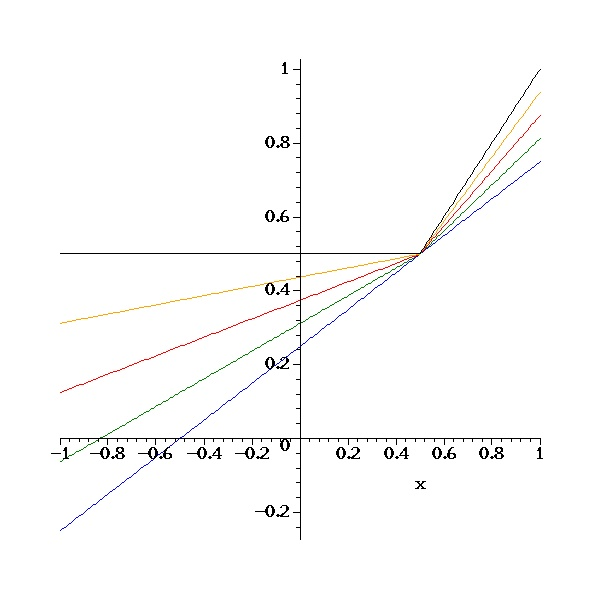
\includegraphics[width=0.5\textwidth,valign=c]{./softmax.jpg}
    \hfill \begin{minipage}{\dimexpr 0.5\linewidth-\columnsep}
        \caption{Representation of the exp-log function for $K = 2$, $i_2 = 1/2$, with $i_1 \in [0, 1]$ and $g \in \{0, 1/4, 1/2, 3/4, 1\}$, from top to bottom, in black, orange, red, green and blue, respectively. With small $g = 1$ it is exactly a linear average, whereas for $g = 0$ it is close to $\max(x, 1/2)$}.
        \label{softmax}
    \end{minipage}
\end{figure}

Derivations of this subsection are available as \href{https://raw.githubusercontent.com/vthierry/braincraft/master/doc/tex/softmax.mpl.out.txt}{{\tt Maple} code}.

\section{Comparing the $h(\cdot)$ sigmoid with other non linearity}

We have $\mbox{h}(x) = \frac{1 + \mbox{tanh}(2 \, x)}{2}$ thus based on the {\tt tanh} non linearity. This corresponds most common activation function
when deriving a rate-based reduced neural network from bio-physical elements  \cite{cessac_neuron_2007}. This is far from being the only choice,
as reviewed in \cite{szandala_review_2020}, and we could have considered, for instance
$\bar{h}$ functions of the form:
\eqline{\begin{array}{|l|c|c|c|c|ll}\hline
 \mbox{Name:} &   \mbox{Tanh} & \mbox{Erf} & \mbox{Arctan} & \mbox{Softsign} \\\hline
 \mbox{Formula:} &
   \frac{1}{2} + \frac{\tan\mbox{h}(2 \, x)}{2} &
   \frac{1}{2} + \frac{\mbox{arctan}\left(\pi  \, x\right)}{\pi} &
   \frac{1}{2} + \frac{\mbox{erf}(\sqrt{\pi} \, x)}{2} &
  \frac{1}{2} + \frac{x}{1 + |2 \, x|} \\\hline
  \mbox{Sharpness:} & & |\mbox{h}(x)| < |\bar{h}(x)| & |\mbox{h}(x)| > |\bar{h}(x)| & |\mbox{h}(x)| > |\bar{h}(x)| \\\hline
  {\cal L}_1 = & 0 & -\frac{\pi  \,\log\left(2\right)-2}{2 \,\pi} & +\infty & +\infty \\\hline
  {\cal L}_0 \simeq & 0 & 0.018 & 0.082 & 0.81 \\\hline
  \kappa_{max} & 1.53 & 1.52 & 2.04 & 4 \\\hline
  \end{array}}
while all profiles are normalized and symmetric, i.e.:
\eqline{\bar{h}(-\infty) = 0, \bar{h}(0) = 1/2, \bar{h}'(0) = 1, \bar{h}(+\infty) = 1, \bar{h}(x) = 1 - \bar{h}(-x)}
and are drawn in the Figure~\ref{sigmoidatan}.
\\ - The {Arctan} and {Softsign} profiles are smoother than the Tanh profile, whereas we are looking here for sharper profiles in order to better approximate the step-function. They also have higher maximal curvatures $\kappa_{max}$ which means that the curvature is more inhomogeneous than for the Tanh profile, and they do not correspond to biologically plausible activation functions \cite{cessac_neuron_2007}, despite the fact they could be of great interest in machine learning \cite{szandala_review_2020}.
\\ - The \href{https://en.wikipedia.org/wiki/Error_function}{error function}, Erf, based profile is very closed numerically from the Tanh profile, with a finite ${\cal L}_1\simeq -0.028$ small distance magnitude, and a ${\cal L}_0 < 2\%$ small distance magnitude, with similar maximal curvatures $\kappa_{max}$ up to $1\%$, and is also quoted as a biologically plausible activation functions \cite{cessac_neuron_2007}. Though its sharpness is a bit better than for the Tanh profile, with a better distribution of the curvature, all algebraic derivations made in this paper would not have as easy as its is now.

\begin{figure}[H]
  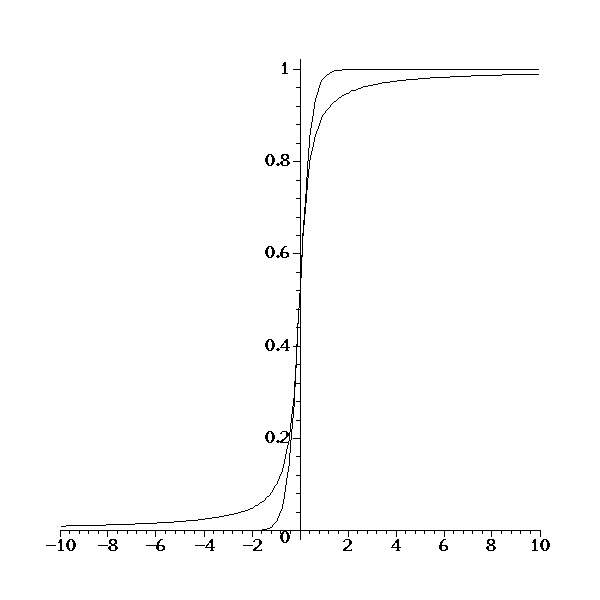
\includegraphics[width=0.5\textwidth,valign=c]{./sigmoidatan.jpg}
    \hfill \begin{minipage}{\dimexpr 0.5\linewidth-\columnsep}
      \caption{Comparison between  the normalized Tanh profile in red, the Erf profile in green, the Arctan profile in blue and the Softsign in orange, i.e., from the sharpest to the smoothest.}
        \label{sigmoidatan}
    \end{minipage}
\end{figure}

Derivations are available as \href{https://raw.githubusercontent.com/vthierry/braincraft/master/doc/tex/sigmoidatan.mpl.out.txt}{{\tt Maple} code}.

\section{Using the braincraft challenge setup}

This documentation allows to use the braincraft challenge for a programmatic implementation, or for a programmatoid/neuronoid implementation using code translator (not yet available).

Here is braincraft challenge original documentation \href{https://github.com/rougier/braincraft/blob/master/README.md}{original documentation}.

You must be familiar with basic {\tt git} usage and basic {\tt python} programming.

\subsection{Installation of the setup}
\begin{enumerate}
\item Connect to {\tt https://github.com} with your login.
\item Go to the \href{https://github.com/vthierry/braincraft}{braincraft challenge} and create a new fork:
\\\centerline{
\includegraphics[width=0.9\textwidth]{tuto1.png}}
\item  Download the repository in SSH read/write mode:
\\\centerline{
\includegraphics[width=0.9\textwidth]{tuto2.png}}
\item In the braincraft local git directory, run \\ {\tt make demo}
\end{enumerate}
Note: You may have to install:
\\ \tab {\tt sudo apt install python3-tqdm}\\
while using a virtual environment, is advised, but not mandatory.

\subsection{Running at the programmatic level}

The bot behavior is defined by:
\\- A state which is a very standard {\tt name $\rightarrow$ value} map, i.e., a dictionary in the {\tt Python} language. It stores all state input, output, and internal state variables, and some parameters.
\\- Two procedures:
\\\tab- {\tt init\_state(state)} called once at the beginning of each run, and
\\\tab-{\tt update\_state(state)} called at each run step.

At the programmatic level, the bot behavior is directly programmed using the target programming language, following this simple example:
\begin{center}\href{https://github.com/vthierry/braincraft/blob/master/braincraft/programmatic_challenge_example.py}{\tt programmatic\_challenge\_example}\end{center}

The \href{https://github.com/vthierry/braincraft/blob/master/braincraft/programmatoid_challenge.py}{{\tt programmatoid\_challenge.py}} source file includes all documented methods and the related API is available here:
\begin{center}\href{https://html-preview.github.io/?url=https://github.com/vthierry/braincraft/blob/master/doc/api/programmatoid_challenge.html}{\tt programmatoid challenge API}\end{center}
  
\subsection{Running at the programmatoid level}

At the programmatoid level, the system is defined by a set of equations of the form: \begin{verbatim}# A tiny example of programmatoid
subs( ## Fixed parameters sequence of constant values
    T = 10, ### The delay
    constantName = constantValue  ### Any other constants
,
[  ## The package options 
  prgm_options = { omega = 10 },
  ## The package equations
  Delay(b, i_t, T),
  a = H(H(b))
])\end{verbatim}

{\bf Note:} The equation list being evaluated in sequence, equations with input must precede equations with output.

This piece of {\tt Maple} code, stored in a file of the form {\tt prgm\_name.mpl} is compiled in the form of straight-line program, with a programmatoid syntax, as defined in this documents.

It is output as a piece of {\tt Python} code and then executed in the desired environment using the:
\begin{center}\href{https://github.com/vthierry/braincraft/blob/master/braincraft/programmatoid_challenge.sh}{\tt programmatoid challenge script}\end{center}
\begin{verbatim}
Usage ./programmatoid_challenge.sh $prgm
  - The programmatoid source is in a $prgm.mpl file.
     - The $prgm name must have a 1, 2, or 3 digit to define the braincraft task number, thus which environment.
  - The compilation output is saved:
    -  In a $prgm.py file for the init_state() and update_state() procedures.
     - In a $prgm.mw file for the maple compilation output.
  - The test is run executing an automatically generated $prgm_test.py file
  - The compilation and execution output is available in $prgm_test.out.wjson (in weak JSON syntax) and $prgm_test.out.html files.
\end{verbatim}

The compilation is parameterized by a set of options given in appendix~\ref{package-options} and is defined using a set of functions given in appendix~\ref{programmatoid-functions} corresponding to all functionnalities defined in this document.

The {\tt \$prgm\_test.out.wjson} output file format uses a dialect of the \href{https://www.json.org/json-en.html}{JSON} syntax, called {\tt wJSON}, for weak-json as \href{https://line.gitlabpages.inria.fr/aide-group/wjson/}{presented here}.

\subsection{Running at the artificial neural network level}

If the {\tt network\_weights} compilation option is raised, is is compiled in the form of a network weights as illustrated\footnote{Shared here by courtesy of R. de Coudenhove, Y. Bendi-Ouis, A. Strock and X. Hinaut.} here:

\centerline{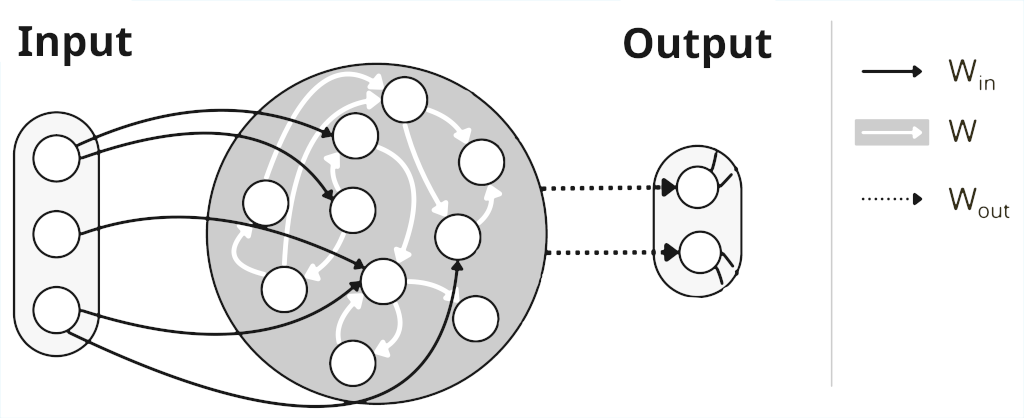
\includegraphics[width=0.9\textwidth]{./res_archi.png}}

and run using the specific  recurrent equations, on input ${\bf I}$ and output {\bf O}, with internal values ${\bf X}$:
\eqline{{\bf X} = h\left({\bf W} \, {\bf X} + {\bf w} + {\bf W}_{in} \, {\bf I}\right), \;\;\; {\bf O} = {\bf W}_{out} \, {\bf X}, \;\;\;\left.{\bf X}\right|_{t = 0} = {\bf 0}}
where:
\\- $W_{out}^{i,j} = \delta_{i = j}$, in words, the output is just a sub-vector of the internal values.
\\- There is no leak, but recurrent connections acting as discrete implementation of a leak.
\\- There is an offset ${\bf w}$ that equivalently corresponds to a a input weight on a constant input.
\\- The non-linearity is a normalized sigmoid.

In fact this compilation option is simply used to verify numerically that such a network is totally equivalent to programmatoid implementation with only neuronoids.

\bibliographystyle{apalike}\bibliography{AIDE}

\appendix \section{Programmatoid package reference}

\subsection{Package and compiler options and outputs}\label{package-options}

\begin{tabular}{|l|l|l|l|} \hline
{\bf Name}                & {\bf Format}                & {\bf Value} & \\ \hline
 &&&\\\multicolumn{4}{|l|}{{\bf Package meta-data.}} \\
{\tt file} 		& string & {\tt path/name.mpl} & \parbox{6cm}{The package source path name.}\\
{\tt name} 	& string & from file name& \parbox{6cm}{The package name.}\\
{\tt excerpt} 	& string & … & \parbox{6cm}{A one or two lines description.}\\
{\tt homepage} & URL & … & \parbox{6cm}{A link to the package, e.g., a git page.}\\
{\tt version} & date & & \parbox{6cm}{The compilation date and time.}\\
{\tt license} & string & {\tt \small CeCILL-C} or … & \parbox{6cm}{The share license. }\\
{\tt author} & Name $<$email$>$ & … & \parbox{6cm}{The person to contact.} \\
 &&&\\ \multicolumn{4}{|l|}{{\bf Compiler parameters.}} \\
{\tt omega}                    & \parbox{3cm}{large float} & 1000 & \parbox{6cm}{The $\omega$ used for {\tt Id()} and {\tt H()} mollification.} \\ &&&\\
{\tt mollification}       & Boolean                   &  false & \parbox{6cm}{Whether {\tt Id()}  and {\tt H()} functions are converted to {\tt h()}.} \\ &&&\\
{\tt networking}  & Boolean                   &  false & \parbox{6cm}{Whether no code, but network's weights is generated.} \\ &&&\\
{\tt python}                & Boolean    &  true    & \parbox{6cm}{If defined, generates a Python piece of code of name {\tt update\_state} with the flattened code.} \\ &&&\\
{\tt inputs}                 & list(name)          &  \parbox{3cm}{r.h.s. variables \\ not in l.h.s.} & \parbox{6cm}{Input variables, user defined or deduced.} \\ &&&\\
{\tt outputs}               & list(name)          &  \parbox{3cm}{l.h.s. variables \\ not in r.h.s.} & \parbox{6cm}{Input variables, user defined or deduced.} \\ &&&\\
&&&\\ \multicolumn{4}{|l|}{{\bf Evaluation parameters.}} \\
{\tt challenge}            & int & & \parbox{6cm}{Challenge number 1, 2, or 3; mandatory} \\ &&&\\
{\tt timeout}              & int & 100 & \parbox{6cm}{Maximum number of iterations.} \\ &&&\\
{\tt runs}                   & int & 1 & \parbox{6cm}{Number of runs, for the evaluation.} \\ &&&\\
{\tt display}               & Boolean & true & \parbox{6cm}{Whether to display animation or not.} \\ &&&\\
&&&\\ \multicolumn{4}{|l|}{{\bf Compiler output.}} \\
{\tt error}                      & string                     & … or not :) & \parbox{6cm}{The error message, if any} \\&&&\\
{\tt source}                     & string                     & & \parbox{6cm}{The parsed input source, without the user options.} \\&&&\\
{\tt expanded}             & string                     & & \parbox{6cm}{The parsed source, with known functions expanded.} \\&&&\\
{\tt flattened}              & string                      & & \parbox{6cm}{The expanded source, with all inner functions generated by new equations.} \\&&&\\
{\tt network[dimension]} & int                         & & \parbox{6cm}{The network internal unit count.}\\
{\tt network[connectivity]} & int                         & & \parbox{6cm}{The network non-sero weight count.}\\
{\tt network[f]}               & list(name)              & & \parbox{6cm}{The unit's non-linearities.}\\
{\tt network[W\_in]}       & matrix                    & & \parbox{6cm}{The input weight's matrix.}\\
{\tt network[W]}             & matrix                    & & \parbox{6cm}{The recurrent weight's matrix.}\\
{\tt network[w]}              & matrix                    & & \parbox{6cm}{The recurrent weights offset, or bias.}\\
{\tt network[W\_out]}     & matrix                    & & \parbox{6cm}{The output weight's matrix.}\\
\hline \end{tabular}

{\bf Note:} All package meta-data and compiler parameters can be overwritten in the source {\tt prgm\_options} first-line.

\newpage \subsection{Programmatoid functions}\label{programmatoid-functions}

For binary variables $\mbox{{\tt b\_$\bullet$}} \in \{0, 1\}$, continuous variables $\mbox{{\tt v\_$\bullet$}} \in [-1, 1]$, and the sigmoid $h(\cdot)$ the following
functions, defined previously, are implemented: \\ \centerline{\begin{tabular}{ll}&\\
  {\tt v\_o = h(v)} & The normalized sigmoid. \\
  {\tt v\_o = H(v)} & Generalized step-function. \\& $\mbox{{\tt v\_o}} \in \{0_{v<0}, 1/2_{v=0}, 1_{v>0}\}$ \\& Converted to {\tt h()}  when the option {\tt prgm["neuronoid"] =  true}.\\
  {\tt v\_o = Id(v)} & Identity function\\& Converted to a neuronoid when the option {\tt prgm["neuronoid"] =  true}.\\
  {\tt b\_o = And(b\_1, …)} & Conjunction with a variable number of binary  arguments.\\& Implements {\tt b\_1 and b\_2 …} \\
  {\tt b\_o = Or(b\_1, …)} & Disjunction with a variable number of binary arguments.\\& Implements {\tt b\_1 or b\_2 …} \\
  {\tt b\_o = Not(b)} & Negation of a binary value. \\& Implements {\tt not b} \\
  {\tt b\_ o = If\_b(b\_1, b'\_1, …, b'\_0)} & Binary conditional expression, \\& Implements {\tt if b\_1 then b'\_1 …}. \\
  {\tt v\_o = If\_v(b\_1, v\_1, …, v\_0)} & Valued conditional expression, \\& Implements {\tt if b\_1 then v\_1 …}. \\
  {\tt v\_o = Exp\_v(v\_1)} & Exponential function approximation \\& Implements $v_1 \in [-1, 1], e^{v_1} \in [1/e, e] \simeq [0.368, 2.718]$ \\
  {\tt v\_o = Log\_v(v\_1)} & Natural logarithm approximation \\& Implements $v_1 \in [1, e], \log(v_1) \in [0, 1]$ \\
  {\tt v\_o = Prod\_v(v\_1, v\_2)} & Multiplication approximation \\& Implements $v_i \in [-1, 1], i \in \{1, 2\}, v_1 \, v_2 \in  [-1, 1]$ \\
  {\tt v\_o = Prod\_b(b\_1, v\_1, …)} & Sum of binary weights values\\& Implements {\tt b\_1 \, v\_1 + …}.\\& Default missing value is $0$.\\
  {\tt v\_o = Softmax(v\_1, …, G)} & Mean-max operator. \\ & $\mbox{{\tt G}} \in [0_{maximum}, 1_{average}]$ controls the mean-max balance.\\
  {\tt Latch\_b(b\_o, b\_i, b\_c)} & Binary memory latch. \\& {\tt b\_o} is the  output, \\& {\tt b\_i} is the input,  \\& $\mbox{{\tt b\_c}} \in \{0_{open}, 1_{latched}\}$ is the control. \\
  {\tt Latch\_v(b\_o, v\_i, b\_c)} & Valued memory latch. \\& {\tt b\_o} is the  output, \\& {\tt v\_i} is the input,  \\& $\mbox{{\tt b\_c}} \in \{0_{open}, 1_{latched}\}$ is the control. \\
  {\tt Bistable(b\_o, b\_1, b\_0)} & Two inputs bi-stable latch. \\& {\tt b\_o} is the  output, \\& {\tt b\_0} resets to $0$, \\& {\tt b\_1} sets to $1$. \\
  {\tt Bistable(b\_o, b\_i)} & One input bi-stable latch. \\& {\tt b\_o} is the  output, \\& {\tt b\_i} is the two-way input.\\
  {\tt Spikeup(b\_o, b\_i)} & Spike generation on input rising front. \\& {\tt b\_i} is the input, which rising front is detected.\\
  {\tt Delay(b\_o, b\_i, T)} & Delayed output. \\& $\mbox{{\tt T}} > 0$ is the delay, in number of global clock event, \\& {\tt b\_o} is the  output, \\& {\tt b\_i} is the delayed input.\\
  {\tt Oscillator(b\_o, b\_c, T)} & Oscillatory output. \\& $\mbox{{\tt T}} > 0$ is the period, in number of global clock event. \\& {\tt b\_o} is the  output, \\& $\mbox{{\tt b\_c}} \in \{0_{stop}, 1_{run}\}$ is the control.\\
\end{tabular}}

\end{document}
